%==============================================================================
\documentclass[11pt,oneside,onecolumn,letterpaper]{article}
\usepackage{times}
\usepackage[paperwidth=8.5in, paperheight=11in,
top=2.5cm, bottom=2.6cm, left=2.58cm, right=2.53cm]{geometry}
%\setlength{\textheight} {9.00in}
%\setlength{\textwidth}  {6.40in}
%\setlength{\topmargin}  {-0.50in}
%%\setlength{\headheight} {0.00in}
%%\setlength{\headsep}     {0.40in}
%\setlength{\oddsidemargin}{-0.010in}
%\setlength{\evensidemargin}{-0.00in}
%==============================================================================
%\usepackage{algorithm}
\usepackage{amssymb}
\usepackage{color,soul}
\usepackage{booktabs}
\usepackage{graphicx}
\usepackage{latexsym}
\usepackage{subfigure}
\usepackage{wrapfig}
\usepackage{amsmath}
\usepackage{amsthm}
\usepackage[hyphens]{url}
\usepackage{pifont}
\usepackage{xcolor}
\usepackage{colortbl}
\usepackage{indentfirst}
\usepackage[lined, boxed, linesnumbered]{algorithm2e}
\usepackage[square, comma, sort&compress, numbers]{natbib}

\newcounter{alg}
\newenvironment{enum-ref}{
\begin{list}%
	{[\arabic{alg}]} {\usecounter{alg}
		\setlength{\leftmargin} {0.25in}
		\setlength{\labelwidth} {0.30in}
		\setlength{\rightmargin}{0.00in}
		\setlength{\topsep}     {0.00in}}
}{\end{list}}

\newenvironment{enum-number}{
\begin{list}%
	{\arabic{alg})} {\usecounter{alg}
		\setlength{\leftmargin} {0.25in}
		\setlength{\labelwidth} {0.30in}
		\setlength{\rightmargin}{0.00in}
		\setlength{\topsep}     {0.00in}}
}{\end{list}}

\newenvironment{enum-nonum}{
\begin{list}%
	{$\bullet$} {
		\setlength{\leftmargin} {0.25in}
		\setlength{\labelwidth} {0.30in}
		\setlength{\rightmargin}{0.00in}
		\setlength{\topsep}     {0.00in}}
}{\end{list}}

\newcommand{\ziming}[1]{%
\begingroup
\definecolor{hlcolor}{RGB}{20, 255, 20}\sethlcolor{hlcolor}%
\textcolor{black}{\hl{\textit{\textbf{Ziming:} #1}}}%
\endgroup
}

\let\chapter\section

%==============================================================================
\pagestyle{plain}
%==============================================================================

\title{Medical Infrastructure Supply Chain (MISC) \\ System Design}
\author{MITRE eCTF 2024\\Team \textbf{Cacti}\\ University at Buffalo}
\date{}



\begin{document}
%%
%=============================================================================
\normalsize


\maketitle
%\date{}

\renewcommand{\thepage}{System Design, Team Cacti, University at Buffalo--\arabic{page}}
\setcounter{page}{1} \normalsize
%
%\renewcommand{\baselinestretch}{1.2}
%\normalsize
%\vspace{0.1in}
%\centerline{\textbf{\Large }}
%\renewcommand{\baselinestretch}{1.0}
%\normalsize

\newcommand{\flagRollback}{\textsf{Rollback}\xspace}

\section{Introduction}
The Medical Infrastructure Supply Chain (MISC) system simulates a supply chain security solution for microcontrollers on a medical device.
Our design consists of three parts: host computer, Application Processor (AP), and Component.
The MISC system includes one AP and two Components connected via an I2C bus.
The host computer is a general-purpose computer communicating with the AP over a serial interface.
The host tools in the host computer send commands to and receive messages from the AP.

The following summarizes the features of the MISC system:
\begin{itemize}
	\item The AP can list provisioned and presented Component IDs.
	\item The whole system will only boot up when all the provisioned Components are present and valid.
	\item The AP can retrieve attestation data from a Component with the correct PIN code.
	\item After replacing a Component,
	the AP needs to be notified the change of a provisioned Component ID.
	\item The integrity and authenticity of communication messages between AP and Component are protected.
\end{itemize}

\section{Security Requirements}

This section defines the security requirements of our design.

The AP and Components must be valid (built by the organizers) for the MISC system to work properly.

\subsection{SR1}
\textbf{The Application Processor (AP) should only boot if all expected Components are present and valid.}
\paragraph{How we address it:}
The AP needs to verify all the present CPs have provisioned IDs and they are valid Components built by the organizers.
We use the public-key cryptography algorithm.
AP holds the public key,
while CP holds the private key.
When the host computer sends the boot command to the AP,
the AP generates a challenge by encrypting a random number using the public key and sends the validation command along with the challenge to one specific Component.
The Component decrypts the challenge using the private key and sends the Component ID along with the decrypted number back to the AP.
The AP then checks the number if it matches the original random number.
If the two numbers are the same,
verification succeeds.
The AP could tell this specific Component is valid.
The AP does this process to all the presented Components.

\subsection{SR2}
\textbf{Components should only boot after being commanded to by a valid AP that has confirmed the integrity of the device.}
\paragraph{How we address it:}
A Component needs to verify if the boot command is given by the valid AP.
We use the RSA algorithm.
AP holds the private key,
while Component holds the public key.
First, the AP sends the boot command to one specific Component.
Then,
this Component generates a random number,
encrypts it with the public key,
and sends the encrypted number to the AP as the challenge.
The AP decrypts the received encrypted number and sends the decrypted plain number back to the Component.
If the received plain number matches the original generated random number,
the Component boots up.

\subsection{SR3}
\textbf{The Attestation PIN and Replacement Token should be kept confidential.}
\paragraph{How we address it:}
The Attestation PIN and Replacement Token will not be stored in plain text or hardcoded in the program (e.g., use the macro generated at the build phase).
The PIN and the Token will be hashed using a keyed-hash algorithm,
and the two hash strings will be stored in the flash memory when the AP board boots for the first time.
Both the AP and the Component hold the same hash key.
After receiving a PIN or a token,
the AP will apply SHA1 to the input,
and compare the hash string with the saved one.
To prevent a brute force attack,
the AP will delay randomly up to 5 seconds after receiving a wrong PIN or token.

\subsection{SR4}
\textbf{Component Attestation Data should be kept confidential.}
\paragraph{How we address it:}
Use AES-128 to encrypt the Component Attestation Data and store it in the flash memory when the board boots for the first time.
To retrieve the data,
a Component uses the same key to decrypt.
To write the plain Component Attestation Data to the I2C buffer,
a Component needs to verify if the request message is from the valid AP.
RSA algorithm and challenge-response mechanism are used for the verification process.
The AP holds the private key,
and the Component holds the public key.
The AP sends a request message to the Component
The Component generates a random number and sends an encrypted number to the AP.
The AP decrypts using the private key and sends back the plain number to the Component.
Verification succeeds if the received plain number matches the generated one.

\subsection{SR5}
\textbf{The integrity and authenticity of messages sent and received using the post-boot MISC secure communications functionality should be ensured.}
\paragraph{How we address it:}
For integrity,
all communications in the I2C bus have the data checksum.
The checksum employs a keyed hash algorithm for the data.
The key is generated from the Global Secret to ensure both the AP and Component have the same key value.
After a Component receives a message or the AP reads a message,
the message will always be validated using checksum.
For authenticity,
a Component needs to validate if the sender is the valid AP before receiving the message,
and the AP needs to validate if a message is read from a valid Component before accepting the read message.
We use the RSA algorithm with two key pairs and the challenge-response mechanism.
For the first key pair,
AP holds the private key,
while Component holds the public key.
For the second key pair,
AP holds the public key,
while the Component holds the private key.
For the scenario of AP sending a message to a Component,
the AP first sends the request message to one specific Component.
The Component sends an encrypted random number to the AP,
and the AP decrypts the received number and sends the transmitted data and decrypted number back to the Component.
The Component can verify if the received number matches the original generated one and receive this message if validation passes.
For the scenario of AP reading a message from a Component,
the AP sends an encrypted random number as a challenge to the specific Component.
The Component decrypts the number and puts the message and decrypted number into the I2C buffer waiting for the AP to read.
The AP reads the data from the Component,
checks if the number matches the original one,
and receives the message if validation passes.


\section{Security Implementations}


\subsection{Build MISC System}
\subsubsection{Build Deployment}
Attackers will NEVER be given access to the Deployment Secrets generated in this step.
\begin{figure}[h]
	\centering
	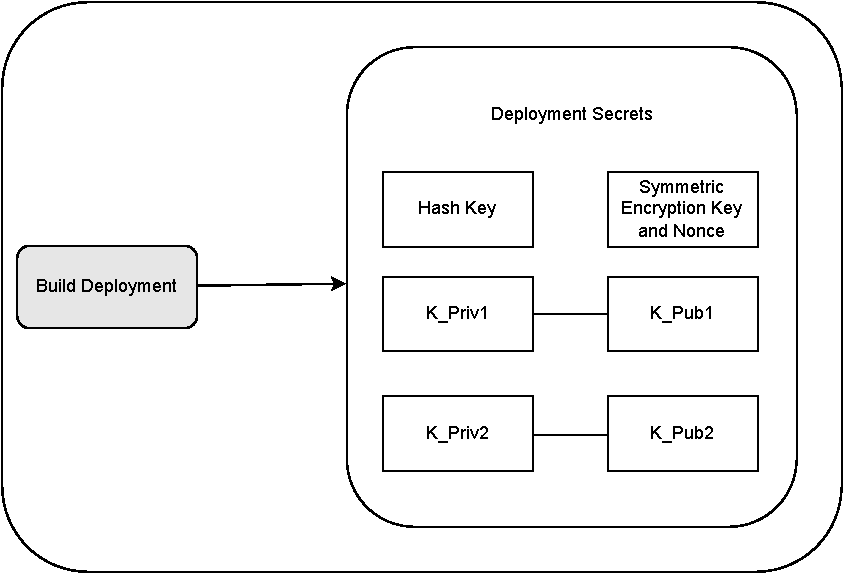
\includegraphics[width=0.65\textwidth]{pics/secret.pdf}
	\caption{Listing Sequence}
	\label{fig:secret}
\end{figure}

Figure \ref{fig:secret} shows the Deployment Secrets.
During the building deployment process,
a Global Secret and two pairs of RSA public and private keys will be generated.
The Global Secret will be shared among the AP and all the Components.
AP will store the private key of \texttt{RSA1} and the public key of \texttt{RSA2}.
Component will store the private key of \texttt{RSA2} and the public key of \texttt{RSA1}.
The \texttt{RSA1} keys are for the AP to validate a Component,
while \texttt{RSA2} keys are for a Component to validate the AP.
We generate the Deployment Secrets randomly when building deployment to prevent the attacker from retrieving it through the source code.

\subsubsection{Build AP and Component Firmware}
To build the AP firmware,
the number of provisioned Components,
provisioned Component IDs,
attestation PIN code,
and replace Token need to be provided.

To build the Component firmware,
the Component ID and attestation data need to be provided.
The attestation data includes location,
date,
and customer name.

\subsection{Load Devices and Booting}
\subsubsection{Load AP and Component Firmware}
The firmware will be loaded by the provided host tool,
teams are not allowed to modify this step.

\subsubsection{First Booting}
Devices will be initialized at the first boot.
The AP will store provisioned Component IDs in plain text,
the private key of \texttt{RSA1},
and the public key of \texttt{RSA2} in the flash memory.
A hash key is generated based on the Global Secret for the keyed-hash algorithm.
The PIN and replace Token will be keyed-hashed,
and the AP stores the hash values in the flash.
The Component stores the private key of \texttt{RSA2} and the public key of \texttt{RSA1}.
An AES-128 key will be generated based on the Global Secret to encrypt the attestation data.
The encrypted data will be stored in the flash.

\subsection{Functionalities}
\subsubsection{Listing}
The Listing functionality checks the provisioned Component IDs of the APs and the IDs of all the presented Components.
As Component IDs are not secrets,
there is nothing to protect during this process.

\begin{figure}[h]
	\centering
	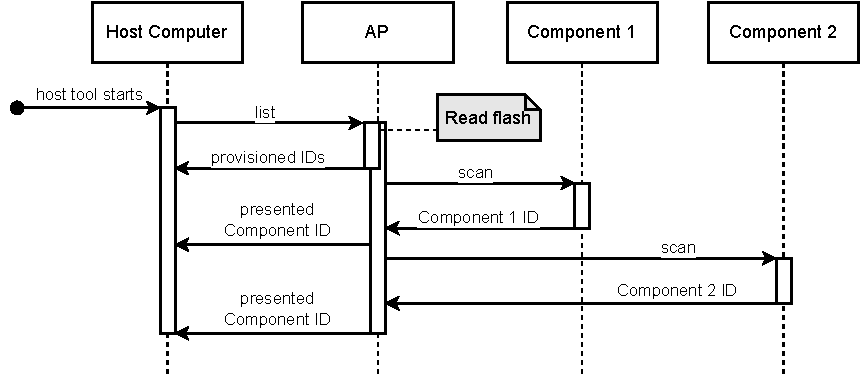
\includegraphics[width=0.8\textwidth]{pics/list.pdf}
	\caption{Listing Sequence}
	\label{fig:functionality_list}
\end{figure}

The process (shown in Figure \ref{fig:functionality_list}) is described as follow:

\begin{enumerate}
	\item The host computer sends the \texttt{list} command through USB to the AP.
	\item The AP reads all the provisioned Component IDs from its flash memory and sends the IDs back to the host computer.
	\item The AP sends the \texttt{scan} command to all the possible Component IDs one by one over the I2C bus.
	\item For one specific ID,
	if the Component with this ID is presented,
	the Component puts the ID value in the I2C buffer for the AP to read.
	\item The AP reads the ID value from this Component and sends the ID value to the host computer as one present Component ID.
	
\end{enumerate}

\subsubsection{Replace}
The Replace functionality is for replacing a Component on the medical device.
The technician in a repair station needs to tell the AP which Component ID is no longer provisioned and what the new Component ID with supplying the correct replacement Token.
The replace Token will be hashed before comparing with the saved Token hash value.

\begin{figure}[h]
	\centering
	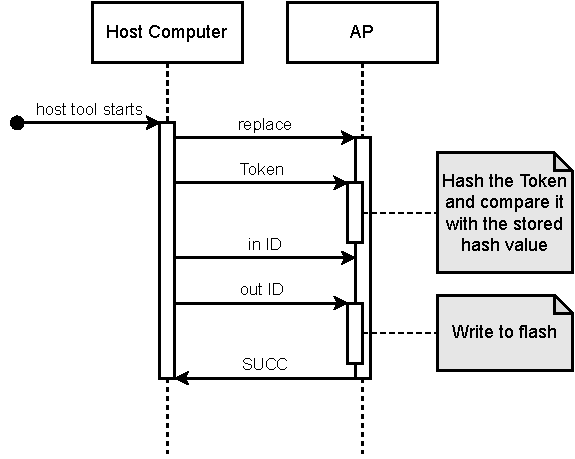
\includegraphics[width=0.55\textwidth]{pics/replace.pdf}
	\caption{Replace Sequence}
	\label{fig:functionality_replace}
\end{figure}

The process (shown in Figure \ref{fig:functionality_replace}) is described as follow:

\begin{enumerate}
	\item The host computer sends the \texttt{replace} command through USB to the AP.
	\item The AP enters the replace mode and waits for the host computer to send the replace Token.
	\item After receiving the Token,
	the AP applies the keyed-hash algorithm to the Token and compares it with the stored hash value.
	All the characters in the hash value are compared one by one.
	The comparison time is always constant no matter if the received Token is correct or not.
	If a wrong Token is received,
	the AP will randomly delay for up to 5 seconds to mitigate brute force and then terminate the replace mode.
	For a correct Token received,
	the AP will wait for the host computer to send the provisioned and new IDs.
	\item The AP modifies the flash memory after receiving the two IDs and sends a success message to the host computer.
\end{enumerate}

\subsubsection{Attestation}
The functionality gets the attestation data from one specific Component by supplying the correct PIN code and the Component ID.
The attestation data is sensitive and encrypted when storing,
so decrypting is necessary when retrieving the data from a Component.
Also,
the PIN code will be hashed before comparing with the saved PIN code hash value.

\begin{figure}[h]
	\centering
	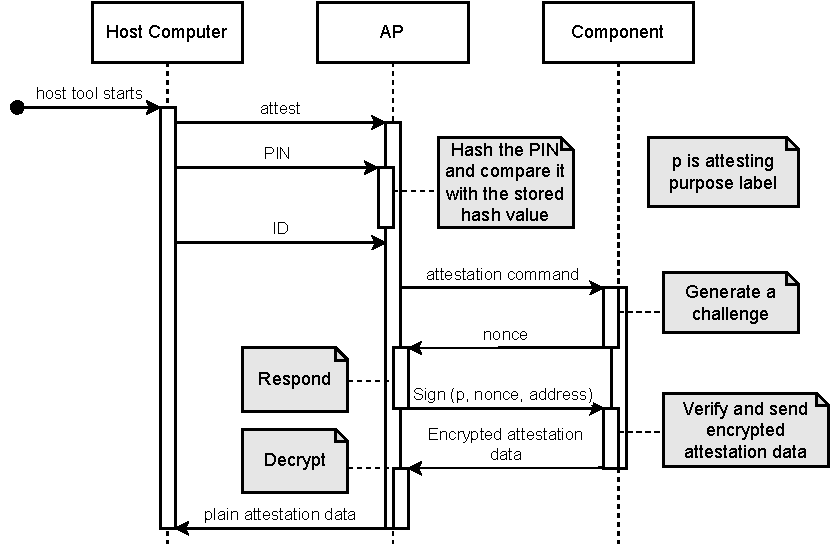
\includegraphics[width=0.8\textwidth]{pics/attest.pdf}
	\caption{Attestation Sequence}
	\label{fig:functionality_attest}
\end{figure}

The process (shown in Figure \ref{fig:functionality_attest}) is described as follow:
\begin{enumerate}
	\item The host computer sends the attest command to the AP
	\item The AP enters the attestation mode and waits for the host computer to send the PIN code
	\item After receiving the PIN code,
	the AP applies the keyed-hash algorithm to the PIN and compares it with the stored one.
	The comparison time is always constant to matter of the PIN correctness.
	The AP will randomly delay for up to 5 seconds to mitigate brute force and then terminate the attestation mode for a wrong PIN.
	When given a correct PIN,
	the AP tries to acquire the attestation data from the specific Component with the ID given by the host computer.
	\item The AP sends the attestation command to the Component.
	\item The Component generates a random number and encrypts it using the \texttt{RSA1\_Pub} key and sends the encrypted number as the challenge to the AP.
	\item The AP decrypts the received message using the \texttt{RSA1\_Pri} key and sends the decrypted number as the response back to the Component.
	\item The Component checks if the received number equals to the original generated number.
	If not,
	the Component sends the verification failure message to the AP,
	and the AP randomly delays up to 5 seconds to prevent brute force and terminate the attestation mode.
	Otherwise,
	the Component retrieves the attestation data,
	decrypts it using the AES algorithm,
	and sends the plain attestation data to the AP.
	\item The AP sends the attestation data to the host computer.
\end{enumerate}

\subsubsection{Boot}
This functionality requires the AP to test if all the provisioned Components are present and valid before the AP boots.
The AP sends commands to all the Components to let them boot,
and the Components must ensure that the boot command is from the valid AP before booting.

\begin{figure}[h]
	\centering
	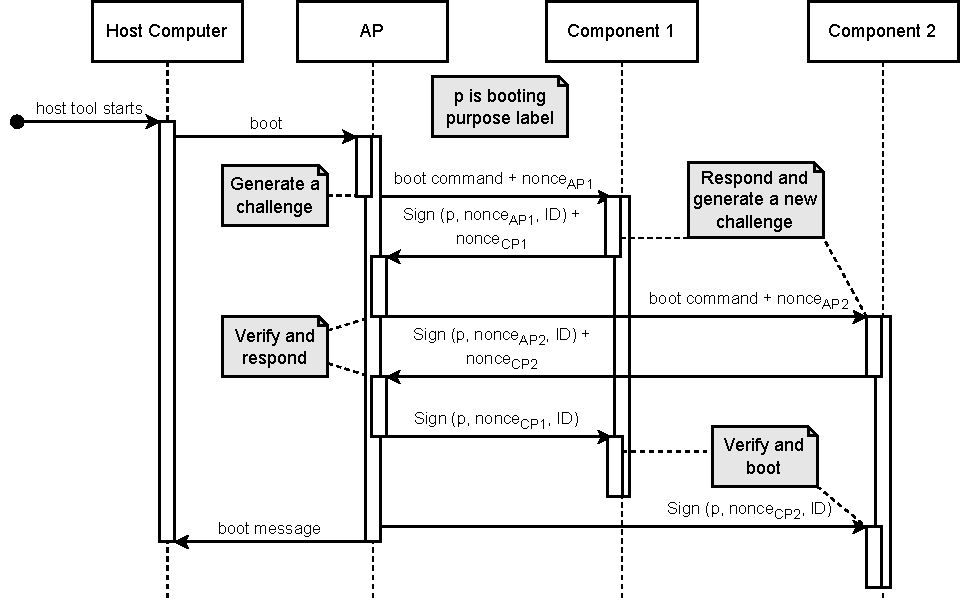
\includegraphics[width=0.8\textwidth]{pics/boot.pdf}
	\caption{Boot Sequence}
	\label{fig:functionality_boot}
\end{figure}

The process (shown in Figure \ref{fig:functionality_boot}) is described as follow:
\begin{enumerate}
	\item The host computer sends the boot command to the AP.
	\item The AP validates all the provisioned Components one by one to check if they are present.
	\item For each provisioned Component,
	the AP generates a random number and encrypts it with \texttt{RSA2\_Pub} key as the challenge.
	It then sends the challenge and validation command message to the corresponding Component.
	\item After receiving the challenge and validation message,
	the Component decrypts the challenge with the \texttt{RSA2\_Pri} key to make up the response and creates a new challenge by using the \texttt{RSA1\_Pub} key awaiting for the AP the read.
	\item The AP reads the response from the Component and validates the response.
	\item If any validation fails,
	the AP will randomly delay for up to 5 seconds to mitigate brute force and terminate the booting process.
	\item If all the Components are present,
	the AP then tries to boot all the them.
	\item For each Component,
	the AP reads the challenge from the Component and decrypts it with the \texttt{RSA1\_Pri} key to make up the response,
	then sends the response back to the Component.
	\item The Component validates the response by checking if it is the same as the original generated random number.
	The Component boots if validation succeeds.
\end{enumerate}

\subsubsection{POST-BOOT Communication}
After the AP and Components boot up,
the communication between the AP and a Component is through the I2C bus.
The AP is the master device,
while the Components are slave devices.
Thus,
the AP can send messages to or read messages from a Component.
However, the Component cannot send messages directly to the AP.
The integrity and authenticity of the communication are necessary.

\textit{Note :} A checksum is used for each sending and reading for communication integrity.

A checksum is calculated by a keyed-hash algorithm with a key generated by the Global Secret.
All the data (except for the checksum) in one communication is a packet,
which is represented as $ Packet = Data + Checksum $.
The $ Data $ may contain a message, command, challenge, and response.
The term message means the real meaningful message the AP intends to send or read.
A checksum calculation includes all the data in a communication,
which is represented as $ Checksum = Hash_K(data) $ ($ K $ is the key).
After the AP or a Component receives a packet,
it will validate the integrity of the packet by using the same keyed-hash algorithm with the same key to calculate the checksum again.
If the calculated checksum does not match the received one,
attack detected and the system terminates this communication.

The checksum generation and validation will be omitted in the following descriptions of the sending and receiving processes.
The descriptions below only focus on validating the AP or a Component for message authenticity.

\begin{figure}[h]
	\centering
	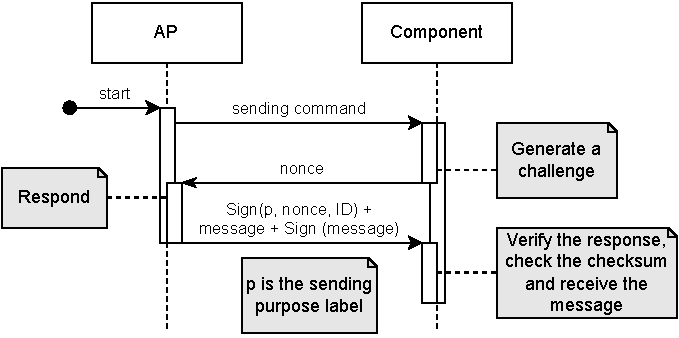
\includegraphics[width=0.7\textwidth]{pics/post1.pdf}
	\caption{Sending Message Protocol Sequence}
	\label{fig:functionality_post1}
\end{figure}

The sending message process is shown in Figure \ref{fig:functionality_post1}.
\begin{enumerate}
	\item The AP sends the sending request command to one specific Component.
	\item The Component generates a random number and encrypts it with the \texttt{RSA1\_Pub} key as the challenge for the AP.
	\item The AP decrypts the challenge using the \texttt{RSA1\_Pri} key as the response for the Component.
	The AP also includes the message along with the response in the packet sent to the Component.
	\item The Component validates the response by comparing the number in the response with the originally generated number.
	If validation is successful,
	the Component receives the message.
\end{enumerate}

\begin{figure}[h]
	\centering
	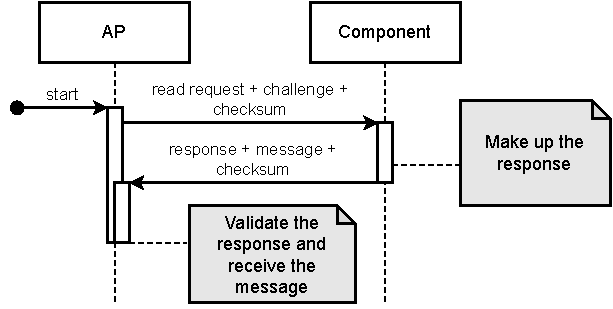
\includegraphics[width=0.7\textwidth]{pics/post2.pdf}
	\caption{Reading Message Protocol Sequence}
	\label{fig:functionality_post2}
\end{figure}

The reading message process is shown in Figure \ref{fig:functionality_post1}.
\begin{enumerate}
	\item The AP generates a challenge by encrypting a random number with the \texttt{RSA2\_Pub} key and sends the read request command along with the challenge to one specific Component.
	\item This Component prepares for the message and makes up the response by decrypting the challenge with the \texttt{RSA2\_Pri} key
	waiting for the AP to read.
	\item The AP read the packet from the Component.
	\item The AP validates the response,
	if validation succeeds,
	it will receive the message.
\end{enumerate}

\end{document}
%==============================================================================
